\documentclass{article}
\usepackage[utf8]{inputenc}
\usepackage{graphicx} %package to manage images
\graphicspath{ {./images/} }

\title{MLE}
\author{panko.aliaksandr }
\date{October 2020}

\begin{document}

\maketitle

\section{Real problem example}
Suppose a data sample is given (ex. the sample of people heights in a particular city).

The task is to make a conclusion about the height distribution in the whole population.

Knowing this information one can, for example, calculate the height of a door in an elevator which fits 99\% of the citizens in this particular location.

\section{Parameter Estimation Idea}
To say that the chosen door height fits at least 99\% of citizens, one should find out the height distribution and after that construct the 99\% theoretical (population) percentile.

What does it mean to find out a distribution? This means 2 things:
\begin{enumerate}
    \item Define distribution family (type)
    \item Find (estimate) a distribution parameters
\end{enumerate}

It is important to understand that one can fit any distribution to any data. Since it is all about the probability, any sample can be from any distribution (except of some obvious cases, where a distribution simply does not allow such values) but just the probability of observing such sample can be incredibly small.

This means that if one picks wrong distribution family (let us say normal distribution instead of student t-distribution) modeling will be biased (in this particular case, one would constantly underestimate probability of observing extreme values aka "fat tails" problem)

Let us assume that we analysed the data (plotted, calculated couple of required statistics) and find out that normal distribution should be the right one.

Now it is time to actually define the distribution. Normal distribution has 2 parameters and only after we know these parameters, we know the distribution.

How to find these values? Moreover, we have just a sample, but want to make a conclusion about the population! This is clear that we cannot find required values precisely, because we do not have data for each person. What we can do it to estimate these values.

Estimate means to say: "most likely these parameters have values ..."

\section{MLE Idea}
In statistics, maximum likelihood estimation (MLE) is a method of estimating the parameters of a probability distribution by maximizing a likelihood function, so that under the assumed statistical model the observed data is most probable.

To understand the idea better let us think about it. The sample data we observe is not likely to be very extreme case, oppositely, they are most likely to be just the most ordinary case. When you travel from home to work, you are not likely to see the whole city of basketball players or dwarfs, isn't it? 

Basically, we want to find such parameter values, under which the data we observe is most probable.
\section{Sample Probability}

So, now the task is to find parameters of already chosen distribution in a way that the probability of observing our already given sample is maximal.

Let us follow the next logical sequence:
\begin{itemize}
    \item Let us threat height as a random variable and our data sample as just a realization of this random variable. Or, in this particular case, we can equivalently say that we have N random variables which are the same (have the same distribution) and the sample is a realization of N random variables.
    \item The next important assumption is independence of all trials (in the first case) or of the all random variables (in the second case). Otherwise one need to use several random variables and know the conditional distributions.
    \item Now we need to find a probability of observing the sample. Let us be more specific at this point. Without loss of generality let us assume the normal distribution. This choice only influence parameters, the cdf and pdf formulas later, but the principle is the same.
    
    \item Let us also assume that we observe sample $s = (x_1,x_2,...x_n)$, where (in our example) $x_i$ is the height of person i.
    \item Now the question comes what is the probability of observing this sample? The answer is 0! Since normal distribution is continuous it is 0! Than how to maximize the probability???
    \item What is can do in this case is to paraphrase the problem: "what is the probability to observe approximately these values?"
    \item Now we need to define "approximately". Without loss of generality let us consider $\pm 3mm$ as approximately equal. Now we have the required interval for a continuous distribution, so we can calculate and maximize the required probability.
    \item Later we can just make this interval even smaller if required.
    \item It is vital to understand that probability density function does not show the probability itself.  $ P(x_1 \in [a_1,b_1]) = \int_{a_1}^{b_1} p(x) \,dx$, where $[a_1,b_1]$ is the required interval 
    
    
\end{itemize}
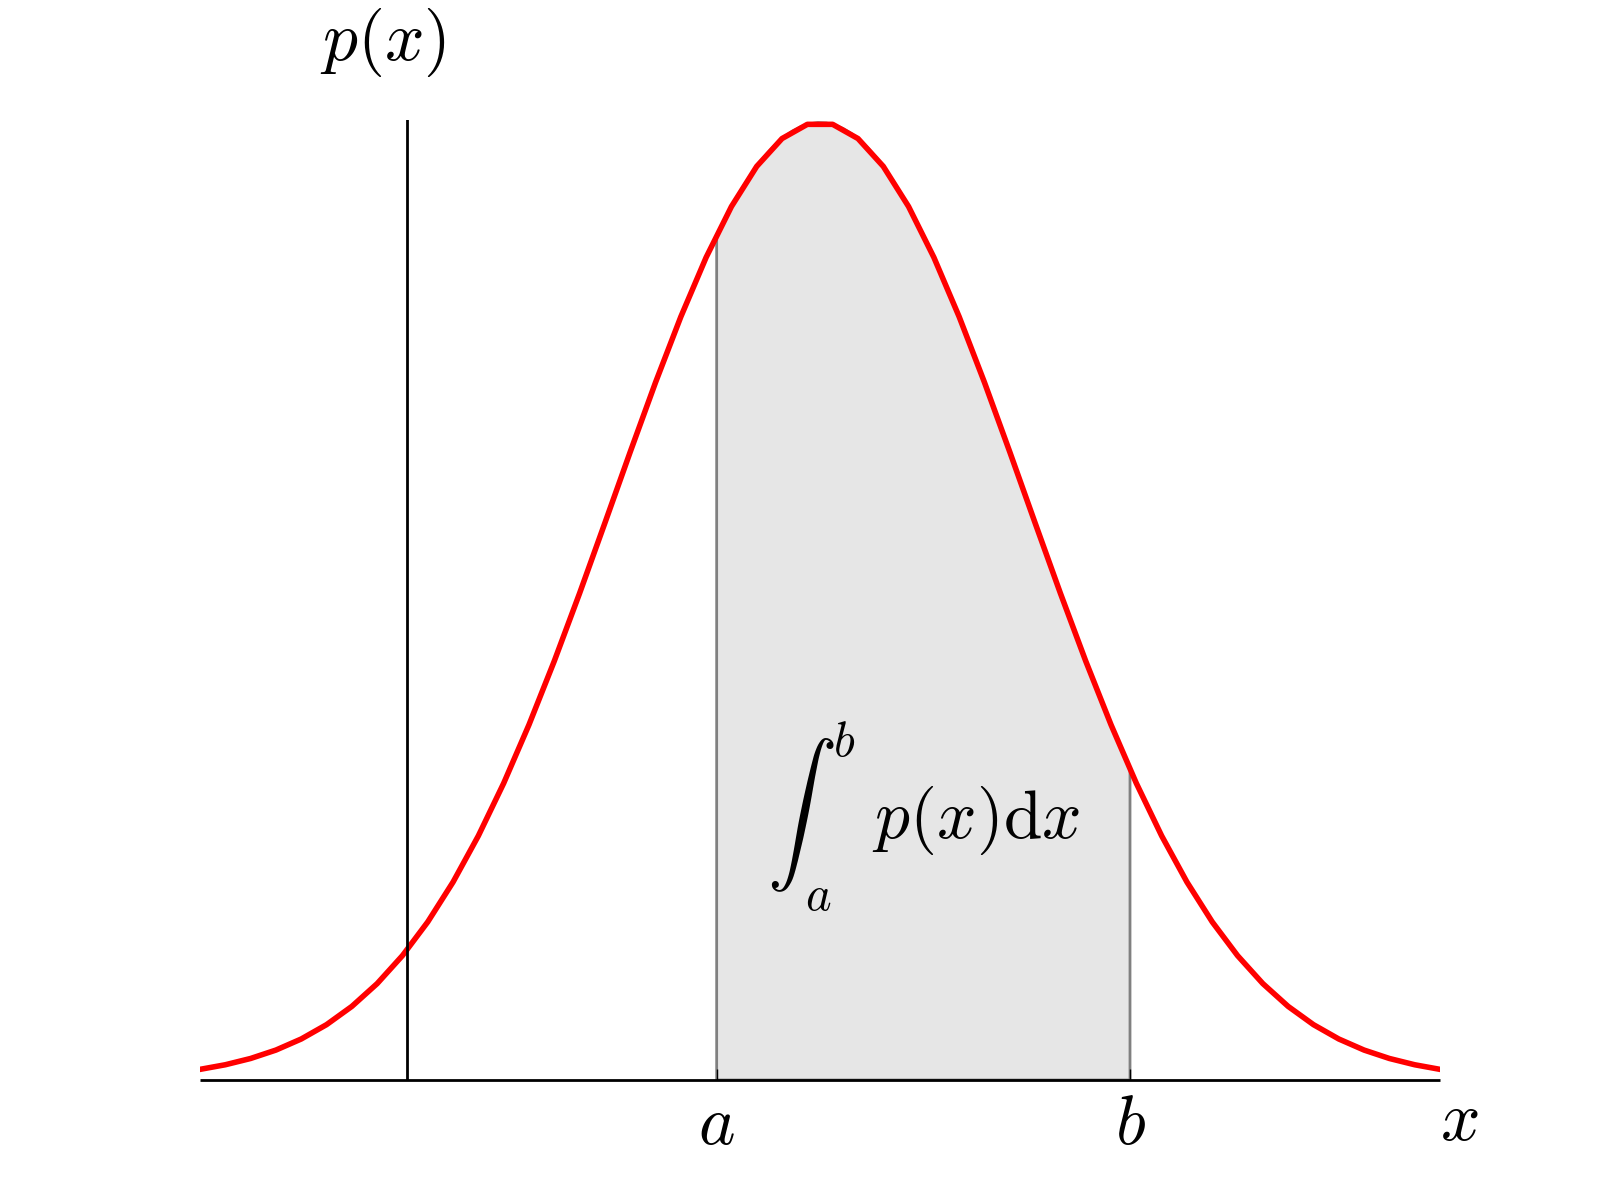
\includegraphics[width=\textwidth]{PDF}

This means that basically we need:
$$ P(x_1 \in [a_1;b_1], x_2 \in [a_2;b_2], ... ,x_n \in [a_n; b_n]) \rightarrow Max $$
Since we assumed independence:
$$ P(x_1 \in [a_1;b_1], x_2 \in [a_2;b_2], ... ,x_n \in [a_n; b_n]) = \prod_{i=1:n}\int_{a_i}^{b_i} p(x) \,dx$$

So, the task is to find a set of parameters $\Theta = (\theta_1,\theta_2,...,\theta_k)$, s.t. $ \prod_{i=1:n}\int_{a_i}^{b_i} p(x) \,dx$ is maximal.

We can simplify it a bit more. Without loss of generality we can pick the same length of interval for all observation: 
$b_1 - a_1 = b_2 - a_2 $ etc.

\section{Likelihood function}
Now is very important part. It sounds pretty intuitively that product of integrals in maximal when product of $p(x_i)$ is maximal (from square of trapezium). But let us prove it:

$$ \int_{a_i}^{b_i} p(x) \,dx = \lim_{\Delta x \rightarrow 0}\sum_{x = a_i}^{b_i}p(x)\Delta x$$

We can take the same $\Delta x$:
$$ \int_{a_i}^{b_i} p(x) \,dx = \lim_{\Delta x \rightarrow 0}\Delta x \sum_{x = a_i}^{b_i}p(x)$$


But $(a_i \rightarrow b_i)$ :
$$ \int_{a_i}^{b_i} p(x) \,dx = \lim_{\Delta x \rightarrow 0}\Delta x p(x)$$ where $x \in [a_i;b_i])$, we can choose $x = x_i$


$$ \prod_{i=1:n}\int_{a_i}^{b_i} p(x) \,dx  = \prod_{i=1:n}\lim_{\Delta x \rightarrow 0} p(x_i)\Delta x$$

So, 
$$ \prod_{i=1:n}\int_{a_i}^{b_i} p(x) \,dx \rightarrow Max  \sim  \prod_{i=1:n}\lim_{\Delta x \rightarrow 0} p(x_i)\Delta x \rightarrow Max$$

Since $\Delta x$ is always positive (by construction) it does not influence argument of the maximum.

$$ \prod_{i=1:n}\int_{a_i}^{b_i} p(x) \,dx \rightarrow Max  \sim  \prod_{i=1:n} p(x_i) \rightarrow Max$$

$\prod_{i=1:n} p(x_i)$ is called the likelihood function.


 The point in the parameter space that maximizes the likelihood function is also maximizes the probability of observing the sample and called the maximum likelihood estimate of a distribution parameters.

\section{Resume}
From a statistical standpoint, a given set of observations are a random sample from an unknown population. The goal of maximum likelihood estimation is to make inferences about the population that is most likely to have generated the sample, specifically the joint probability distribution of the random variables ${\displaystyle \left\{y_{1},y_{2},\ldots \right\}}$, not necessarily independent and identically distributed. 

To find these estimates we need to find argument of maximum of the likelihood function.
\end{document}
